\documentclass[11pt,ngerman]{article}
\usepackage{geometry}
\usepackage[T1]{fontenc}
\usepackage[utf8]{inputenc}
\usepackage{babel}
\usepackage{lmodern}%get scalable font
\usepackage{titling}
\usepackage{relsize}
\usepackage{biblatex}
\usepackage{hyperref}
\usepackage{paralist}
\usepackage[table, dvipsnames]{xcolor}
\usepackage{booktabs}
\usepackage{setspace}
\usepackage{float}
\usepackage{graphicx}

\geometry{a4paper, top=25mm, left=25mm, right=25mm, bottom=20mm,
    headsep=10mm, footskip=12mm}

\renewcommand{\arraystretch}{1.5}

\pretitle{\begin{center}\linespread{1.5}\huge}
    \posttitle{\par\end{center}\vspace{0.5em}}

\begin{document}

    \title{SWEN1\\Praktikum 02\\
        \vspace{1cm}
        \small{ZHAW  School of Engineering\\Klasse: IT18tb\_zh}
        \vspace{1.5cm}
    }
    \author{
        Huber, Patrick\\
        \small{huberpa4@students.zhaw.ch}
        \vspace{1.5cm}
    }
   \date{\today}

    \maketitle
    \newpage

    \tableofcontents
    \listoffigures
    \newpage

    \section{Domänenmodell}

    \subsection{Problembeschreibung}
    Sie erhalten den Auftrag, eine Software für ein Buchungssystem für Hotels zu entwickeln. Mit dem Auftraggeber haben Sie ein ausführliches Gespräch geführt und dabei die folgenden Notizen gemacht:\\
    \begin{itemize}
        \item Der Kunde (der, der die Ferien bucht) wählt zuerst das exakte Datum, die Länge der Ferien und die Destination und erhält darauf hin die verfügbaren Hotels mit den Gesamtpreisen.
        \item Pro Destination besitzt der Betreiber des Buchungssystems Vertragsverbindungen mit einer gewissen Anzahl Hotels. Es werden nur Angebote von solchen Hotels dem Kunden vorgelegt.
        \item Die Vertragsbeziehungen regeln insbesondere die Verkaufsmarge (Anteil am Übernachtungspreis, den die Buchungsplatform erhält)
        \item Die Angebote der Hotels werden in Echtzeit von den jeweiligen Hotel-Reservationssystemen abgefragt. Ihre Software muss diese also nicht verwalten.
        \item Hat der Kunde ein Hotel gebucht, werden dem Kunden noch zusätzliche Hoteldienstleistungen angeboten. Diese sind spezifisch für ein bestimmtes Hotel und können über die Jahreszeit und die Verfügbarkeit variieren.
        \item Die Bezahlung erfolgt ausschliesslich per Banküberweisung
        \item Die Benutzerschnittstelle richtet sich an geübte Computerbediener und soll alle relevanten
        Informationen auf einmal zeigen, auch wenn dadurch die Übersichtlichkeit leidet.
        \item Die Benutzerschnittstelle richtet sich an geübte Computerbediener und soll alle relevanten
        Informationen auf einmal zeigen, auch wenn dadurch die Übersichtlichkeit leidet.
    \end{itemize}
    \clearpage

    \subsection{Hotelbuchungssystem}

    \begin{figure}[H]
        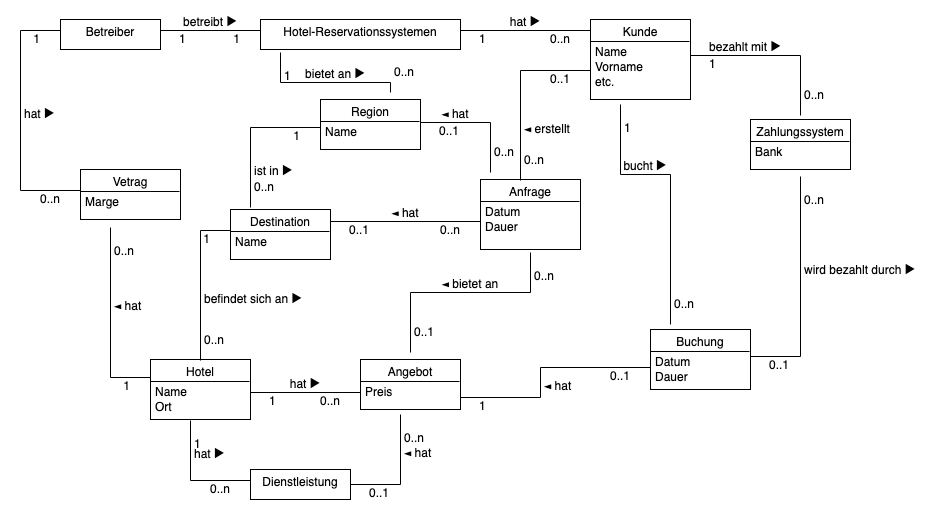
\includegraphics[scale=0.50]{HotelBuchungsSystem.png}
        \caption{Domänenmodell Hotelbuchungssystem}
    \end{figure}


\end{document}

